\section{Visão Geral}\label{5-estudo-de-caso-visao-geral}

A especificação WSDL, utilizada nesta prova de conceito, descreve um serviço web no domínio cinematográfico. A \figurename~\ref{fig:estudo-de-caso-grafo-wsdl} ilustra o grafo para a especificação WSDL utilizada nesta prova de conceito. A fim de simplificar o processo, a especificação WSDL contém apenas uma operação, cujo objetivo é a busca de filmes em um dado repositório. Este repositório e a implementação das operações em si não são relevantes para este trabalho. A operação de busca de filmes tem como resultado uma lista de filmes. Um filme é composto por uma lista de premiações (\texttt{Awards}), uma lista de atores (\texttt{Actor}), uma lista de produtoras (\texttt{Producer}), uma lista de diretores (\texttt{Director}), um país (\texttt{Country}), um gênero (\texttt{Genre}), um nome (\texttt{Name}) e um ano de lançamento (\texttt{Year}). Uma premiação (\texttt{Award}) é composta pelo nome (\texttt{Name}) e pelo ano da premiação (\texttt{Year}). Um ator (\texttt{Actor}) é composto pelo primeiro nome (\texttt{FirstName}) e pelo sobrenome (\texttt{LastName}). Uma produtora (\texttt{Producer}) é composta pelo nome (\texttt{Name}). Um diretor (\texttt{Director}) é composto pela data de nascimento (\texttt{DateOfBirth}), pelo primeiro nome (\texttt{FirstName}) e pelo sobenome (\texttt{LastName}). Um país (\texttt{Country}) é composto pelo nome (\texttt{Name}). Por fim, um gênero (\texttt{Genre}) é composto pelo nome (\texttt{Name}).

\begin{landscape}
    \begin{figure}[h]
        %\resizebox{\textwidth}{!}{
            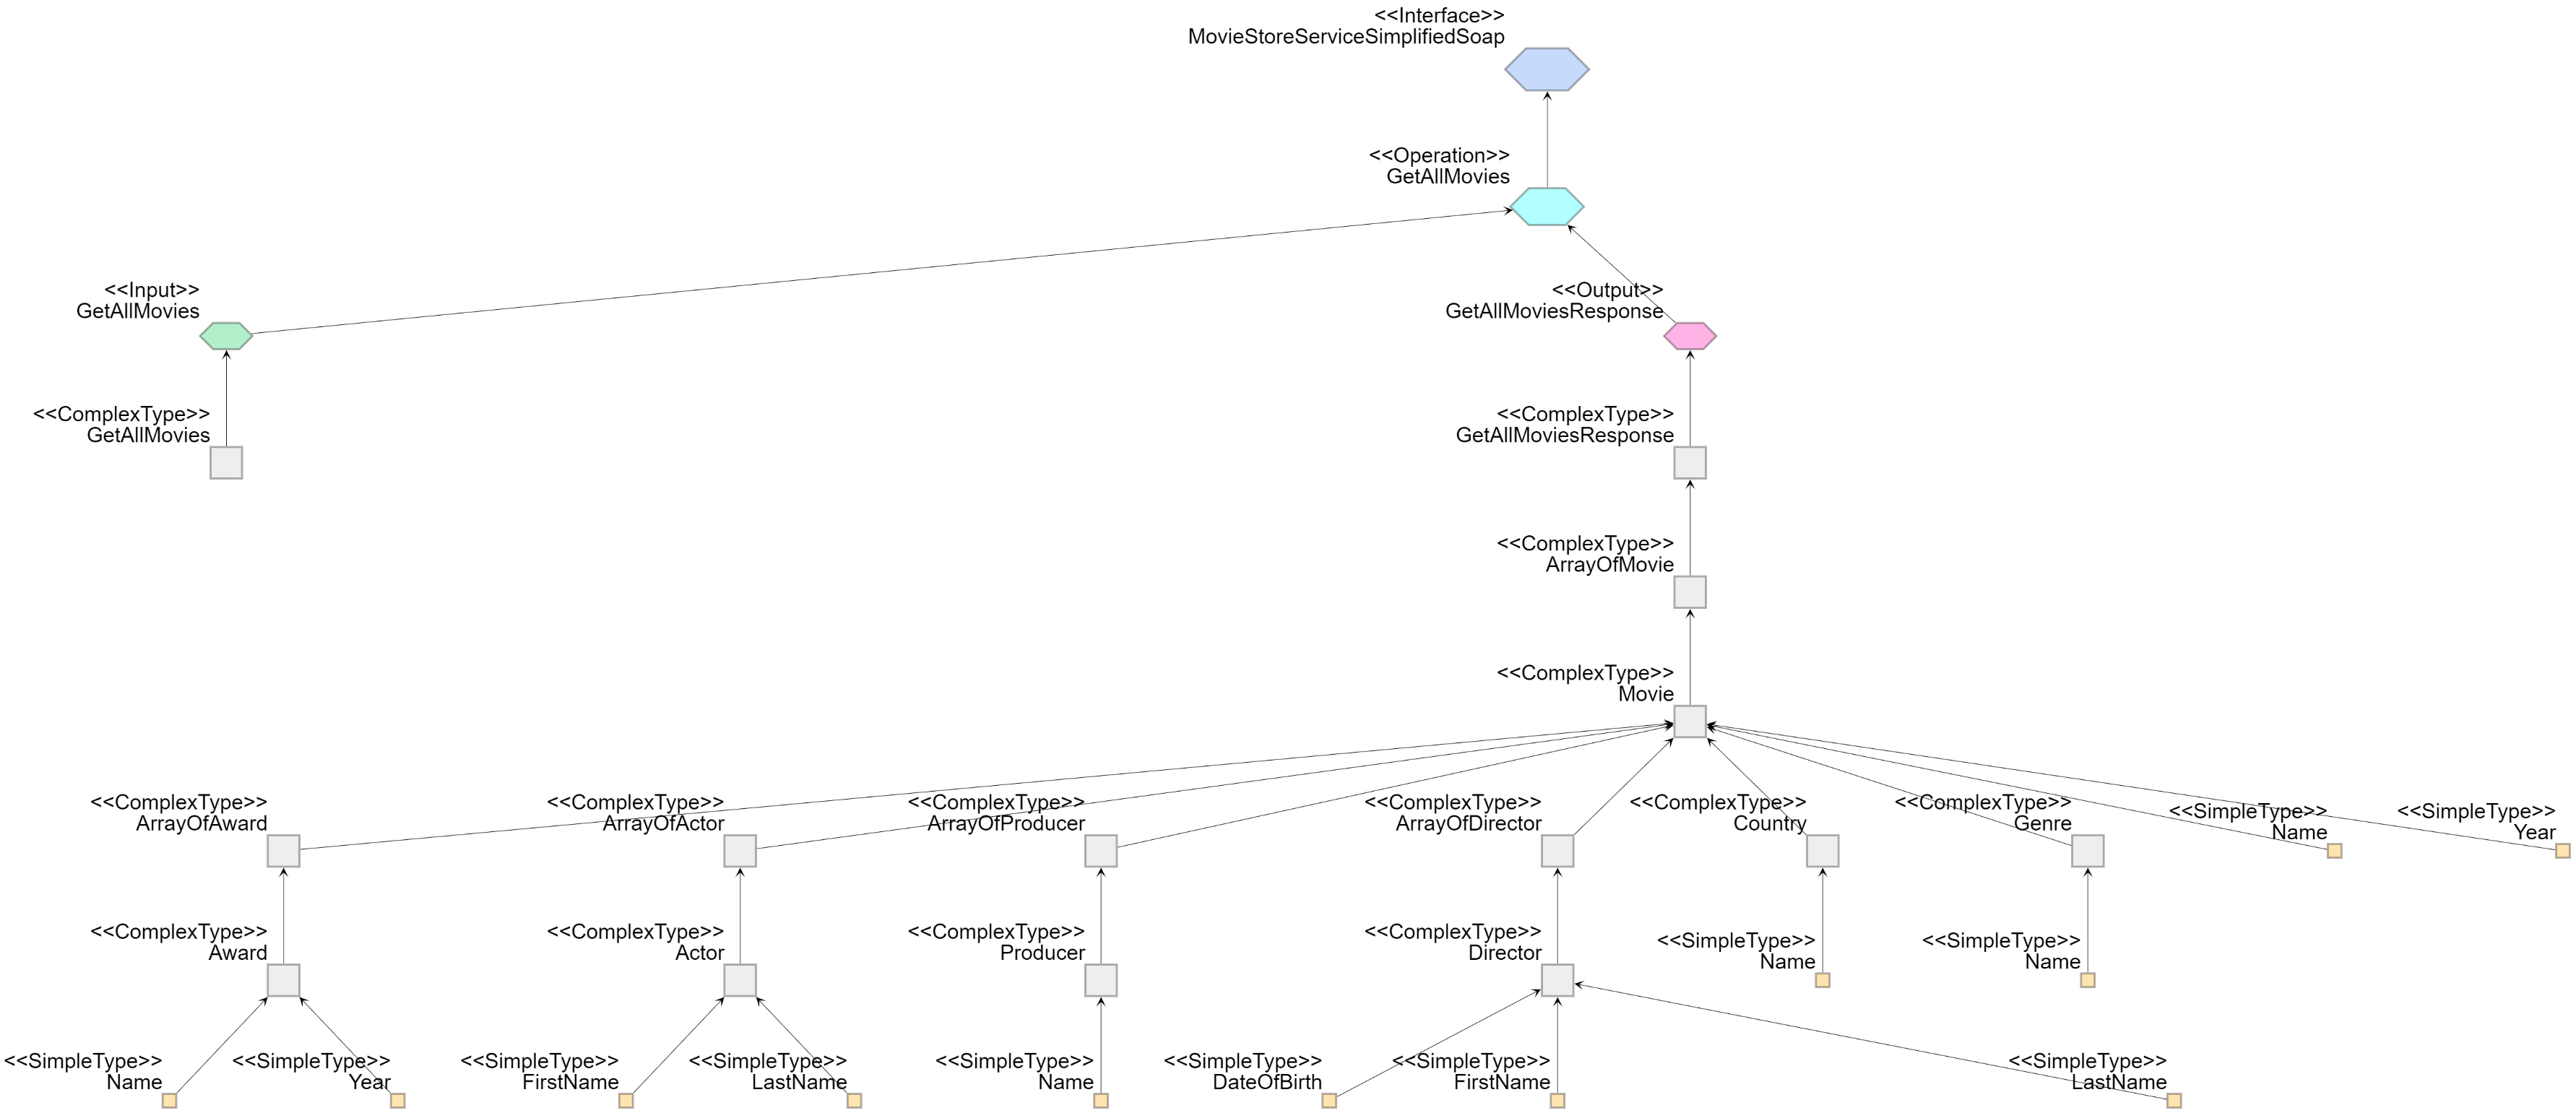
\includegraphics[scale=0.65]{5-grasews-estudo-de-caso/imagens/estudo-de-caso-grafo-wsdl.png}
        %}
        \centering
        \caption[Grafo da especificação WSDL utilizada na prova de conceito]{\textbf{Grafo da especificação WSDL utilizada na prova de conceito.}}
        \label{fig:estudo-de-caso-grafo-wsdl}
    \end{figure}
\end{landscape}

O documento de especificação WSDL deste processo possui o nome \break\texttt{MovieStoreServiceSimplified2.0} e encontra-se disponível no endereço \url{https://raw.githubusercontent.com/mlcalache/wsdls/master/MovieStoreServiceSimplified2.0.wsdl}. Adicionalmente, esta especificação WSDL está disponível no Anexo \ref{anexo-WSDL-estudo-de-caso}.

A fim de termos todos os artefatos necessários para apresentar este processo, em conjunto com a especificação WSDL, utilizamos a ontologia OWL \texttt{MovieOntology}~\cite{MOVIEONTOLOGY-2019}. A ontologia contém hierarquias de conceito para categorização de filmes que permitem a apresentação amigável de descrições de filmes. Esta ontologia foi desenvolvida pelo Departamento de Informática da Universidade de Zurique.

Neste processo, dois usuários trabalharam colaborativamente na anotação semântica da especificação WSDL. O primeiro usuário, denominado \texttt{Usuário A}, consiste de desenvolvedor de serviços web, enquanto que o segundo usuário, denominado \texttt{Usuário B}, consiste de um especialista no domínio cinematográfico. O \texttt{Usuário A} é possui o conhecimento especializado na tecnologia envolvida no desenvolvimento de serviços web semânticos e acerca de quais elementos WSDL/XSD devem ser anotados. Entretanto, o \texttt{Usuário A} não possui o conhecimento especializado no domínio e, consequentemente, acerca de quais termos da ontologia que devem ser utilizados na anotação. Eis que surge o importante papel do \texttt{Usuário B}, que auxiliou o \texttt{Usuário A} na solução de dúvidas e na finalização de tarefas para a anotação semântica da especificação WSDL.